\section{Model vodenja z adaptivnim genom}

Problem se pri genetskem algoritmu lahko pojavi, ko se število ovc na pašniku močno zmanjša, saj so parametri ves čas enaki, odvisni le od začetnega števila ovc. Parametre želimo prilagajati trenutnemu stanju na pašniku, številu ovc, psov in še čemu, kar bi lahko koristilo uspešnosti vodenja črede. Celo bolje bi bilo, če bi se ovčarji lahko naučili česa novega, izvirnega, česar naš model ne predvideva niti ob spreminjanju parametrov. Želimo mu dati čim bolj proste roke pri izbiri smeri in hitrosti.

Za to bomo uporabili metode umetne inteligence, ki nam omogočajo učenje čim boljših potez v določenem trenutku. Z vodenjem črede s pomočjo spodbujevanega učenja so se ukvarjali tudi avtorji člankov~\cite{obstacles} in~\cite{sarsa}. Ker je naš program pripravljen v programu Unity, smo se odločili za uporabo paketa ML Agents, ki temelji na spodbujevanem učenju, konkretno na PPO algoritmu. V tem poglavju bomo predstavili ta izbrani algoritem.

\subsection{Spodbujevano učenje}

Spodbujevano učenje je osredotočeno na interakcijo med agentom in okoljem, pri čemer agent maksimizira nagrade, ki jih dobi iz okolja, ko v danem stanju naredi neko potezo~\cite{reinforcement}, kot lahko vidimo na sliki~\ref{fig:reinforcement}. Agent je hkrati učenec in odločevalec. Tekom učenja skrbi za ravnotežje med raziskovanjem nepoznanega in izkoriščanjem pridobljenega znanja.

\begin{figure}[ht]  % ali t za na vrhu ali h! za točno tukaj
	\centering
	\includegraphics[width=0.7\textwidth]{../poglavja/images/reinforcement.pdf}
	\caption[Agent in okolje pri spodbujevanem učenju]{Interakcije med agentom in okoljem.} % narejena je s programom Inkscape
	\label{fig:reinforcement}
\end{figure}

Model sicer pogosto temelji na markovskem procesu odločanja, za katerega bi lahko narisali graf stanj in povezav med stanji z verjetnostmi prehodov, ampak za algoritme spodbujevanega učenja ne potrebujemo poznavanja tega grafa, saj ga algoritem sam raziskuje in se uči najboljših odločitev v raziskanem prostoru brez računanja in pomnjenja samega grafa.

Okolje modela je določeno s stanji $s \in S$, potezami $a\in A(s)$, ki so agentu na voljo v stanju $s$, pripisanimi numeričnimi nagradami $r(s, s^\prime, a) \in R$ ob izbrani potezi $a$ in spremembi stanja iz $s$ v stanje $s^\prime$ ter verjetnostmi stanj $P(s^\prime \vert s, a)$ doseženih iz stanja $s^\prime$ z uporabo poteze $a$. Prav ta verjetnost in vrednosti nagrad so nam običajno neznane.

Agent se med možnimi potezami odloča na podlagi svoje strategije izbire akcij. Med učenjem posodablja strategijo $\pi(a, s)=P(a\vert s)$, ki predstavlja verjetnost izbire poteze $a$ v stanju $s$ tako, da je pričakovana vsota nagrad v prihodnosti največja, torej maksimiziramo vrednostno funkcijo izbranega stanja $s$ ob uporabi izbrane strategije
\begin{align}
V^\pi(s) &= E\lbrack r_{t+1} + \gamma r_{t+2} + \gamma^2r_{t+3} + \ldots\vert s_t=s, \pi\rbrack, \label{eq:value}
\end{align}
kjer sledimo trenutni strategiji $\pi$ in je $\gamma\in\lbrack 0, 1)$ diskontni faktor, ki uravnoteži pomen trenutne nagrade in prihodnjih. Funkcija $V(s)$ oceni dolgoročni obet uporabe strategije $\pi$ iz trenutnega stanja, pri čemer da manjšo težo oddaljenim nagradam. Tako se agent načeloma izogiba potezam, ki mu bodo dolgoročno škodovale in se raje odloča za tiste, ki mu obljubljajo večjo nagrado v krajšem času. Pri učenju pa je pomembno, da agent tudi raziskuje po prostoru stanj. K temu ga spodbudimo z naključnimi potezami z verjetnostjo $\epsilon$. Ta parameter je običajno najprej nastavljen na neko začetno vrednost med 0 in 1, potem pa pada skozi čas proti 0. S tem agent najprej predvsem raziskuje, potem pa vedno bolj izkorišča svoje znanje, ki si ga je pridobil. Vseeno pa se lahko ujame v lokalnem optimumu.

Agent mora oceniti lastnosti okolja, predvsem verjetnost prehodov med stanji $P(s^\prime\vert s, a)$, da lahko oceni vrednosti stanj. Na principu spodbujevanega učenja z nagradami in kaznimi se v veliki meri učijo tudi človeški možgani. Razvitih je že mnogo algoritmov za učenje optimalne strategije, kot so TD-Learning, Q-Learning, SARSA, globoko Q-učenje, PPO in drugi. Paket ML Agents uporablja algoritem PPO, zato si tega nekoliko podrobneje oglejmo.

\subsubsection{Optimizacija z bližnjo strategijo}

Motivacija za optimizacijo z bližnjo strategijo (Proximal Policy Optimization - PPO) je vprašanje, kako kar najbolj izboljšati strategijo na podlagi trenutne, brez da bi zaradi slučajne velike nagrade pomotoma stopili predaleč in povzročili nenaden padec uspešnosti strategije. PPO za vrednosti parametrov nima omejitev, ampak ima omejitev le na velikosti koraka, s katerim spremenimo parametre. Omejitev je postavljena z namenom, da je nova strategija dovolj podobna prejšnji, saj bolj zaupamo vrednostim parametrov blizu prejšnje strategije, ker nočemo uničiti naučenega na podlagi posamezne ocene.

PPO je algoritem, ki se uči napovedovanja pričakovanih nagrad, da se tako odloča za najbolj obetavne poteze v danem stanju. S pomočjo gradientnega spusta spreminjamo vektor parametrov $\theta_k$ in s tem strategijo $\pi^{\theta_k}$, ki je odvisna od tega vektorja. Vektor parametrov si lahko predstavljamo kot vektor uteži v nevronski mreži. Pri tem moramo stanje in potezo nekako numerično predstaviti modelu. Poleg nevronske mreže, ki izračuna verjetnost neke poteze na podlagi stanja, definiramo tudi vrednostno funkcijo $\hat{V}^{\phi_k}(s)$, ki oceni vrednost prihodnjih nagrad z uporabo nevronske mreže, ki jo naučimo ocenjevati pričakovane nagrade na podlagi stanja. Tudi ta funkcija mora biti odvedljiva in odvisna od vektorja parametrov $\phi_k$. 

PPO je za razliko od Q-Learning in nekaterih drugih algoritmov spodbujevanega učenja primeren tudi za zvezna prostora možnih potez in stanj. Razvil ga je Schulman iz OpenAI s sodelavci. Predstavljen je v članku~\cite{ppo-clanek}. Algoritem je po rezultatih primerljiv drugimi trenutno najboljšimi algoritmi spodbujevanega učenja, njegova prednost pa je predvsem v relativno enostavni implementaciji in nastavljanju parametrov algoritma.

Pri tem algoritmu definiramo tudi primerjalno funkcijo
\begin{align}
L(s,a,\theta_k,\theta) = \min\left(\frac{\pi_{\theta}(a|s)}{\pi_{\theta_k}(a|s)}  A_t^k(s,a),~g(\epsilon, A_t^k(s,a))\right), \label{eq:lclip}
\end{align}
kjer je $\theta_k$ trenutni vektor parametrov strategije (v našem primeru uteži nevronske mreže), $\theta$ izbrani vektor parametrov strategije, ki ga primerjamo s trenutno strategijo, $A_t^k$ je ocenjena donosnost poteze ob času $t$, $\epsilon$ je parameter, ki omejuje spremembo strategije, običajno med 0.1 in 0.2 ter
\begin{align}
g(\epsilon, A) = \Big\{
\begin{array}{ll}
(1 + \epsilon) A & A \geq 0 \\
(1 - \epsilon) A & A < 0.
\end{array}
\end{align}

Donosnost poteze je enaka $A_t^k = V(s_t) - \hat{V}^{\phi_k}(s_t)$. Torej predstavlja razliko med točno vrednostjo vrednostne funkcije izračunane na podlagi dejanskih nagrad, ki ni samo ocena in njeno oceno izračunano po formuli pridobljeni na podlagi preteklega znanja z vektorjem parametrov $\phi_k$, ki se jih prav tako sproti učimo za boljše ocenjevanje pričakovanih nagrad.

PPO posodablja strategijo na sledeč način:
\begin{align}
\theta_{k+1} = \arg \max_{\theta} \underset{s,a \sim \pi_{\theta_k}}{{\mathrm E}}\lbrack
L(s,a,\theta_k, \theta)\rbrack, \label{eq:posodobi}
\end{align}
običajno z več koraki stohastičnega gradientnega spusta za maksimizacijo primerjalne funkcije. Za lažjo optimizacijo je priporočljivo, da sta vrednostna funkcija in strategija odvedljivi. Če je donosnost poteze pozitivna, oziroma je višina nagrad nad pričakovanji, verjetnost izbire poteze $a$ pa je po strategiji $\pi_\theta$ večja kot prej, raje izberemo to strategijo, saj želimo verjetnost dobre poteze povečati. Prav tako zmanjšamo verjetnost slabe poteze. Funkciji $min$ in $g$ pa služita temu, da damo strategijam z relativno razliko med verjetnostjo izbire poteze $a$ v primerjavi s staro strategijo večjo od $\epsilon$ enako primerjalno vrednost. S tem se izognemo navduševanju nad velikimi vrednostmi primerjalne funkcije, ki bi nas potegnile daleč od trenutne strategije, ki ji dolgoročno bolj zaupamo, saj ni odvisna le od posamezne uspešnosti simulacije, ki je lahko le posledica šuma, ki ga povzroča velika variabilnost vrednosti nagrad. S tem se strategija ne more dramatično spremeniti, lahko pa se poveča vrednost vrednostne funkcije. V algoritmu~\ref{alg:ppo} si lahko postopek podrobneje ogledamo.

\begin{algorithm}[ht]
	\caption{PPO}
	\label{alg:ppo}
	\begin{algorithmic}[1]
		\State Vhod: začetni parametri strategije $\theta_0$, začetni parametri vrednostne funkcije $\phi_0$
		\For{$k = 0,1,2,...$}
		\State Zberi množico izvedenih simulacij ${\mathcal D}_k$ z uporabo strategije $\pi_{\theta_{k}}$.
		\State Izračunaj dobljene nagrade $(r_t)_{t=0}^T$ za vsako simulacijo.
		\State Izračunaj ocene donosnosti $(A_t^k)_{t=0}^T$ temelječ na vrednostni funkciji $\hat{V}_{\phi_{k}}$.
		\State Posodobi strategijo s pomočjo primerjalne funkcije:
		\begin{equation*}
		\theta_{k+1} = \arg \max_{\theta} \frac{1}{|{\mathcal D}_k| T} \sum_{\tau \in {\mathcal D}_k} \sum_{t=0}^T L(s_t, a_t, \theta_k, \theta),
		\end{equation*}
		običajno preko stohastičnega gradientnega spusta.
		\State Popravi vrednostno funkcijo z regresijo, da bo čim manjša napaka vsote kvadratov:
		\begin{equation*}
		\phi_{k+1} = \arg \min_{\phi} \frac{1}{|{\mathcal D}_k| T} \sum_{\tau \in {\mathcal D}_k} \sum_{t=0}^T (V(s_t) - \hat{V}_\phi(s_t))^2,
		\end{equation*}
		običajno preko algoritma gradientnega spusta.
		\EndFor
	\end{algorithmic}
\end{algorithm}


\subsection{Adaptivni gen}

Pri učenju modela smo najprej poizkusili na način, da bi ovčarju dali proste roke, da se odloča o smeri in hitrosti na podlagi opazovanj. Poizkušali smo z različnimi funkcijami za nagrajevanje, veliko različnimi opazovanimi vrednostmi in celo z demonstracijami, kar pomeni, da smo algoritem najprej učili brez, da bi ta poskušal z naključnimi potezami, ampak s potezami, kakršne je izbiral ovčar z optimalnim genom iz genetskega modela. Če smo dali ovčarju popolnoma proste roke, se ni uspešno naučil niti sam, celo z eno samo ovco. Ta prostor stanj je bil prevelik, da bi ga agent uspešno spoznal in se iz njega česa naučil. Običajno se v različnih virih ML Agents uporablja za bolj enostavne probleme. Poizkusili smo še z manj svobodnim modelom. Ta model smo poimenovali \textit{adaptivni gen}.

Ideja je, da damo ovčarju le nekaj opazovanih vrednosti, on pa se odloči za najboljši gen znotraj dovoljenih meja za vsako vrednost v genu. Gen je definiran enako kot v poglavju~\ref{genetski}. Adaptivni gen bi moral imeti celo boljše rezultate kot optimalni gen iz genetskega algoritma, saj ima ta model še več svobode in vključuje tudi možnost, da se nauči enakih genov kot druga dva modela, če jih vmes ne spreminja. Vemo, da model naučen z genetskim algoritmom deluje, dovolj bi ga bilo le izboljšati. Ovčar naj se nauči izbire gena iz le nekaj osnovnih opazovanih lastnosti. Ker pa je učenje precej zamudno, smo se odločili le za Ginellijev model ovc in le za enega ovčarja na naključno veliki čredi med 1 in 10 ovcami, saj je ta model bolj podoben naravnemu obnašanju ovc, ovčar pa je imel probleme le sam, s sodelovanjem pa je model precej uspešen že z genom dobljenim z genetskim algoritmom. Večje črede pa se mu žal ni uspelo naučiti voditi niti v več urah.

\subsection{Naša implementacija modela}

Model se odloča vsakih 20 korakov, kar pomeni na 0,4~s. Med posameznimi odločitvami uporablja gen, ki ga je nazadnje izbral. Trajanje simulacije $T$ smo navzgor omejili na 750 izračunov gena (300~sekund oziroma 5~minut), kar je več kot tri minute z namenom, da se lahko uči vodenja tudi, če je za zbiranje potreboval več časa. Za primerni vrednosti parametrov modela sta se izkazali vrednosti $\epsilon=0,2$ in $\gamma=0,99$. Pred učenjem smo naredili 128 simulacij za pospešitev učenja na podlagi demonstracij. Za izbiro poteze se je model naučil uteži za nevronsko mrežo s 5 plastmi po 512 nevroni.

\subsubsection{Nagrajevanje}

Ovčar dobi nagrado veliko $\frac{1}{20T}$ vsakič, ko center črede (GCM) premakne staji bliže, kot je bil center blizu staji kadar koli pred tem znotraj simulacije. V vsakem časovnem koraku pa dobi prav tako kazen, ki ga spodbuja k hitrejšemu reševanju problema. Kar pomeni, da ovčar dobi kazen v primeru, da črede ne pripelje bliže staji, sicer ne dobi ničesar.

Ko spravi zadnjo ovco v stajo dobi še $4(\frac{T - t}{T})^2$ nagrade za uspešno opravljeno nalogo, kjer je $t$ čas ob zaključku simulacije. Z višino nagrade ga spodbujamo k hitrejšemu vodenju.

\subsubsection{Opazovanje vrednosti}

Stanje, v katerem je ovčar, definiramo s številom ovc na pašniku, deležem pobeglih ovc glede na trenutni delež dovoljenih pobeglih ovc, razliko med GCM in stajo ter ovčarjem in stajo v smeri $x$ in $z$. Uporabimo izračunane vrednosti v tem in prejšnjem koraku posodabljanja gena.

Poleg tega ovčar opazuje tudi oddaljenost objektov v smereh devetih žarkov razvrščenih okrog njega s skupnim kotom $120^\circ$. Pri tem lahko loči med ovco in ograjo oddaljeno največ 50~m. Na sliki~\ref{fig:zarki} si lahko ogledamo razvrstitev žarkov.

\begin{figure}[ht]  % ali t za na vrhu ali h! za točno tukaj
	\centering
	\includegraphics[width=0.8\textwidth]{../poglavja/images/zarki.png}
	\caption[Predstavitev prostora z žarki]{Predstavitev prostora z žarki. Ovčar lahko prepozna objekt in določi razdaljo do njega.} % narejena je s programom Inkscape
	\label{fig:zarki}
\end{figure}

